
\chapter{Case Päikky}

This thesis approaches the research problem through a real-life case study in which an offline support was implemented to an already existing system. This chapter describes the basics of that system and the use cases of it. The technical characteristics and domain knowledge of the system which are important for understanding the functionality of the offline support are opened up in more depth. 

The reasoning behind the decisions done regarding the implementation of the offline support are described.


%% ------------------------------------------
\section{System Description}

The system under the analysis is \textit{Päikky}, a solution for daycare personnel & daycare children’s parents for planning the needed daycare and providing passage control of the children (and for the personnel) on the kindergarten. 

Päikky is a collaborative web application for daycare personnel and children's parents to plan and coordinate daily activities in kindergarten. Päikky also provides functionality which helps kindergarten personnel to coordinate the daily activities on the kindergarten and communicate with the children's parents.
%Application under our case analysis is Päikky, a solution for daycare personnel & daycare children’s parents for planning the needed daycare and passage control of the children on the daycare. 

Päikky consists of four parts:

\begin{enumerate}
	\item \textit{Kindergarten UI}, mobile-first single-page application used for logging children in/out to kindergarten, referenced as \textit{the application} later on,
	\item \textit{Family UI}, single-page application used by parents when planning children daycare time
	\item \textit{Manager UI}, single-page application used by kindergarten management 
	\item \textit{backend}, Grails-powered server that implements REST API and other services used by the Päikky UI's.
\end{enumerate}

Under the hood \textit{Manager UI} and \textit{Family UI} are actually both on the same codebase, and from technical point of view they are a single web application. From user's standpoint they are although inseparable, since despite sharing the same architecture the layout and functionalities are completely different. Contrary to the \textit{Kindergarten UI} they are designed to be used primarily from desktop clients. 

In this thesis we are focusing mainly on the \textit{Kindergarten UI}, which is the tool used on daily basis by the kindergarten nurses for tracking the attendance on their care group. Some emphasis is also on the backend due to its major role on the system's overall view.

\begin{figure}[t]
\begin{center}
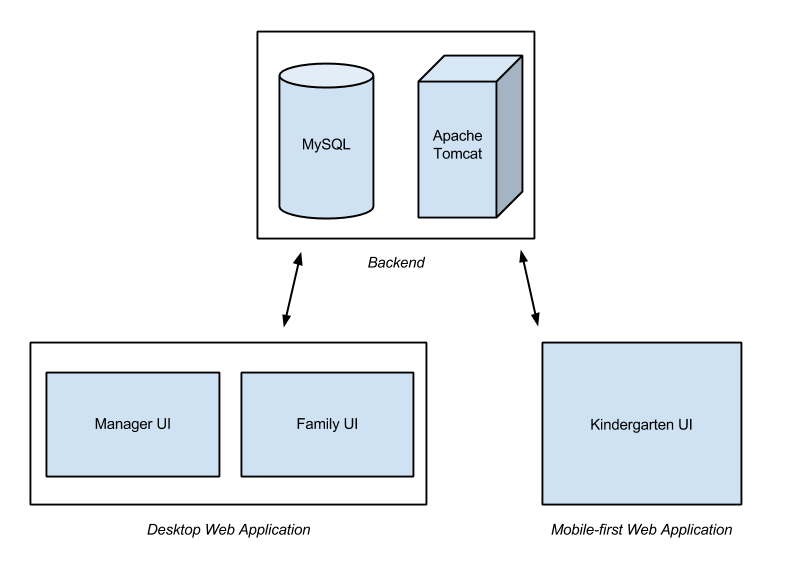
\includegraphics[width=1\textwidth]{assets/architecture.png}
\end{center}
\caption{The high-level architecture of Päikky}
\label{fig:architecture}
\end{figure}



% ##
\subsection{Backend}

The backend is the web server of Päikky which holds all the master data of the system. It serves the HTML content and other resources (graphical assets, JavaScript files, Cascading Style Sheets) to the other modules of Päikky. The backend also implements a REST API which from the other modules requests and alters the data on the system. The abilities the API offers differs between the type of the user's account, but in practice all of the data can be modified via it. Data is exchanged between the backend and the UI modules of Päikky as a JSON objects.

Currently the backend is operated as a single virtual machine on the Amazon Web Services cloud. The data is stored on a single \textit{MySQL} database. The backend is \textif{multitenant}\footnote{Principle where single instance serves multiple tenants}: single instance serves multiple municipalities and kindergartens. 


%-REST API requista tänne jotain, että mitä hä? Hox linkissä tämä-implementation-research (vai tulisko tää tohon ylempään sectioniin?)

% <IMPR tarvisko jotain lisää kertoa vielä bäkkäristä? mitä? hitusen tynkäkappale just ny>



% ##
\subsection{Kindergarten UI}

Kindergarten UI is the part of Päikky which is used daily by the kindergarten nurses. From the Kindergarten UI nurses can also see elaborate information about the children, including allergies and persons who are allowed to pick them up, have parents allowed the children to be photographed. Nurses can also easily see the contact information for each child. Updating this information is also possible. % They can also monitor the overall presence of persons in the kindergarten, including both children and other nurses.

On Kindergarten UI the key activity for nurses is to log in children (and the other nurses) when they arrive at the kindergarten and log them out when a child or nurse leaves. This activity is repeated tens of times per day. To do this conveniently nurses are equipped with \textit{Android} smart phones. The marking of goings and leavings has to be done in order to replicate the presence status from the real world to the Päikky system. Since monitoring attendance and in the future creating bills for provided daycare is based on the presence data generated by logging the personnel in and out, it is crucial that this activity can be achieved successfully under any kind of condition. Doing this activity should also be as effortless and simple as possible for the nurses so that it would get done at the exact moment when the actual event happens on the kindergarten. 

The simplicity requirement goes for every other aspect of the system: the Päikky users' demography is a very mixed crowd. The kindergarten nurses' age can be anything from 18 to 65. Because of the age variation also the ability and the starting level to use a digital service via smartphone varies a lot. Taking the easiness of usage is also one of the key principles behind Päikky's user interface and interaction design. It is also one of the unique selling points of the company behind Päikky, the \textit{MukavaIT}\footnote{http://mukavait.fi}: \textit{"using IT systems shouldn't be hard or unpleasant"}.

Based on the plans done by parents on the \textit{Family UI}, nurses can see how many and who of the children they are expecting to appear for each day. If the parents have to change the already existing plans with short notice, automated message is sent to the nurses stating the change, and the plans visible for the child relating the case gets updated in real time. Nurses can also see the exact amount of children and nurses present at the kindergarten for any given time.

As stated above, the attendance of nurses can also be tracked with the Kindergarten UI. With the \textit{Manager UI} it is also possible to plan shifts for the nurses. Combined with the planned attendance data of children done by the parents, this makes Päikky a powerful tool for organizing the kindergarten's daily schedule and ensuring that there are always enough nurses present to take care on the children. This is important since required nurses/children ratio is dictated by law in Finland. % IMPR tarttisko tähän lakiviitteen?

From technical point of view looking the Kindergarten UI is a single-page web application (introduced on the Section~\ref{sec:spa}) created to be used primarily with mobile devices. The libraries the application consists of are: %

\begin{enumerate}
	\item \textit{Backbone}\footnote{\href{http://backbonejs.org/}{http://backbonejs.org/}}, \textit{Model-View-Template} –framework providing the – wait for it – backbone for the application,
	\item \textit{Marionette}\footnote{\href{http://marionettejs.com/}{http://marionettejs.com/}}, library of common design and implementation patterns for Backbone,
	\item \textit{RequireJS}\footnote{\href{http://requirejs.org/}{http://requirejs.org/}}, module loader and dependency manager,
	\item \textit{Underscore}\footnote{\href{http://underscorejs.org/}{http://underscorejs.org/}}, functional programming inspired library for utility functions,
	\item \textit{jQuery}\footnote{\href{http://jquery.com/}{http://jquery.com/}}, utility library for DOM manipulation,
	\item \textit{Moment}\footnote{\href{http://momentjs.com/}{http://momentjs.com/}}, time and timezone handling library. 
\end{enumerate}


The method of data synchronizing between Kindergarten UI clients and the backend is \textit{polling}. Each client sends checksums of its attendance data to the backend on a regular interval, and if the backend calculates different checksum for the data requested, new data is returned to the clients. This means that if child is logged in to kindergarten with device A, it can take as long as the configured interval for the device B to receive that information. The current interval is 45 seconds. Before the interval was only 20 seconds, but as the user amount increased the current infrastructure which Päikky is run on couldn't handle the amount of requests invoked by that interval. 

The devices and browsers targeted during the development process and which  were delivered to the kindergartens by the client organization were \textit{Samsung Ace 3 Style}'s and the latest stable version of the \textit{Chrome} browser. The devices uses mobile broadband connection as their access method in reaching the Internet. Usually each of the kindergarten's care groups have at least one dedicated device at their disposal. Large groups might have two devices. 

The usual – and most of the time the only – usage environment for Kindergarten UI are the kindergartens around Finland which are using Päikky. The application is used in both outside and inside. Kindergartens can be located practically anywhere, and the mobile reception can vary a lot between different kindergartens. In some locations the coverage and experienced connection quality can be at par with physical broadbands, but the locations with the worst reception are very challenging from the connection speed and latency point of view looking. It is not unusual for the kindergarten to be located on a remote location where getting 3G connection is more of an exception than standard behaviour. % no pitäsköhä tälle olla joku viite:-D


% ##
\subsection{Presence Model}

% -> Presence type/state (kumpi?!), Presence state transfer tms, check implementaation viimeinen kappale

As the primary functionality for Päikky is the monitoring and planning of the attendance of the people on the kindergarten, one of the most essential data models is also the one implementing this feature. The backbone for holding and handling this data is Päikky's \textit{presence model}. In brief presence model is an entity which indicates a range of time when person has had a certain status. These entities are persisted by the Päikky backend on the database.

There are different \textit{purposes} for presences: \textit{actual, plan change, plan} and \textit{default plan}. Each presence has always a single purpose. The purposes are similar for both children and for nurses. Each of the purposes exists on their own domain, resulting in a layered construct of presences for each person. The \textit{actual} presences are the most significant, while the \textit{default plan} is the least significant. This is visualized on the Figure~\ref{fig:presencemodel}. Person's presences with same purpose may never overlap. For single person there can be only one or zero presences per purpose at any given time.

\begin{figure}[t]
\begin{center}
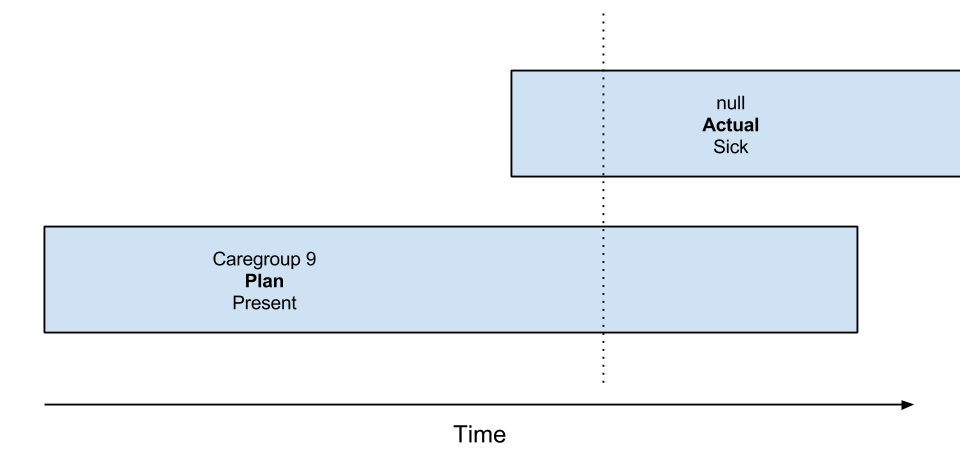
\includegraphics[width=0.8\textwidth]{assets/presencemodel.png}
\end{center}
\caption{The presence model of Päikky.}
\label{fig:presencemodel}
\end{figure}


Each presence also has a single type. The ones used the most are \textit{present, sick} and \textit{day off.} These basic types are the same for children and nurses, but nurses also have a extended set of types indicating specialized reasons for not being at the kindergarten. For example these types includes likes of different cases of sick leaves, trainings and holidays. In this thesis we are concentrating at looking the system primarily from the children's presence markings perspective.

A single presence always belongs to a single person. The presence always has a start time and an end time. There is one special case when presence doesn't need to have an end time (it is then set null on the database): if the purpose for presence is \textit{actual} and that presence is the latest ongoing presence for the person. For example when person is logged in to the daycare on the morning, a new presence entity is created. For this presence start time is set to be the time when he/she arrived to the kindergarten, and end time is left null. This means that this presence is \textit{active} for the current person, indicating ongoing activity. When the person leaves the kindergarten the active presence's end time is set to be the leaving time. If their state is otherwise altered, the active presence is ended and new presence entity with the new type is created. The ending time for the previous presence is the same as the starting time for the new presence. 



% ###
\subsection{Presence Status and Presence State Machine}
\label{subsec:presencestate}

Based on the presence entities of an individual person a \textit{presence status} for they can be determined on any time point. For example if person has a planned presence for the day but they has not arrived at the kindergarten yet, the status would be transcribed as "not yet present" indicating that this person will be present later on today. Mutually if the person has been today at the kindergarten but has already left, their status would be "left for today". The status mechanism is implemented for providing more information about the current attendance status for the kindergarten personnel, in contrary to what simple boolean "present / away" statuses would implicate.

Within presences sharing the same presence purpose, there is a set of rules of allowed state transitions. These rules can be visualized as a \textit{finite-state machine} that shows the possible transitions from different status into another. 

% https://docs.google.com/drawings/d/17hQD7BYT4MUqfRaWlX0ykesfond-cTlAmOQ9Zn9LFQk/edit
\begin{figure}[t]
\begin{center}
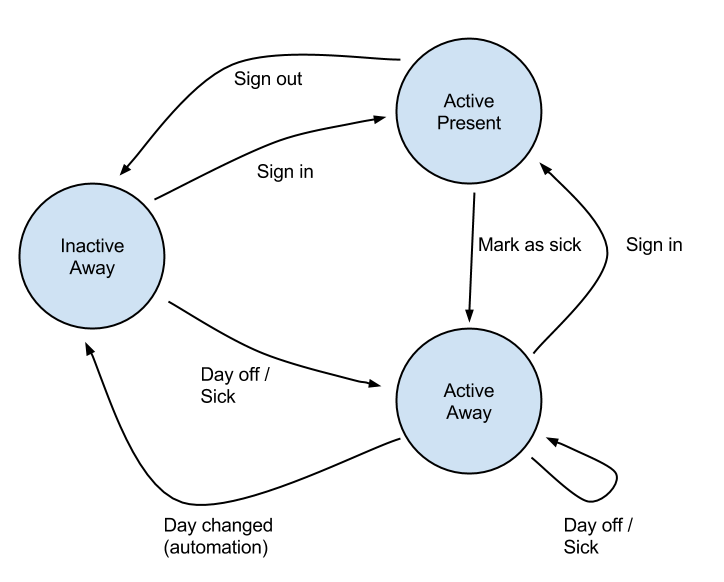
\includegraphics[width=0.8\textwidth]{assets/statemachine.png}
\end{center}
\caption{Presence State Machine. For visualizing purposes this state machine is a simplified version from the one actually implemented on Päikky}
\label{fig:statemachine}
\end{figure}

The Figure~\ref{fig:statemachine} describes a simplified version of Päikky's state machine. In this finite-state machine each state indicates two things: is there an active ongoing presence entity for the individual person which has "actual" as the presence purpose ("Inactive~/~Active" on the visualization), and if the current state means that the person is physically present at the kindergarten or not ("Present~/~Away").

Based on the allowed state transitions different kind of buttons for altering the presence state are shown on the person's profile UI. For the most straightforward example if the person is already present on the kindergarten, only a \textit{sign out} button is shown. Since signing in a person already present on the kindergarten is prohibited by the presence state machine, the button \textit{sign in} button is therefore also hidden from the UI. This can be seen on the Figure~\ref{fig:child-profile}. 


\begin{figure}[t]
\begin{center}
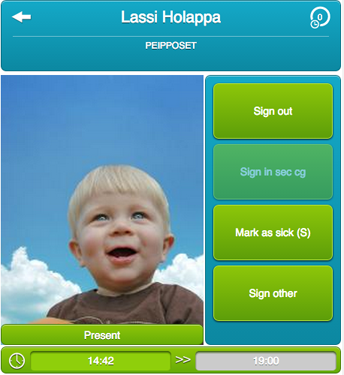
\includegraphics[width=0.5\textwidth]{assets/child-profile.png}
\end{center}
\caption{Screen capture from a child's profile on the Kindergarten UI}
\label{fig:child-profile}
\end{figure}







%% -------------------------------
\section{Need for Offline Support on Päikky}
\label{sec:need-for-offline-support}
% pitäisikö tässä esittää jotenkin selkeämmin, että nämä on Peten kautta validoituja ajatuksia?

% jari: "kilpailutus päättyi tammikuun lopussa muistaakseni (20.1.), koekäytön piti alkaa maaliskuussa jne"

Päikky's development was originally started with creating of a \textit{MVP version}\footnote{Minimum Viable Product} of the product, which was used in validating the business case of the idea. Therefore it had only a thin feature set, covering only the most essential features needed for the application. According to the client organization's CEO, the need for some level of of offline support was noticed on an early phase of the system's development. The marking of persons' status was also recognized to be the key activity already at the start of the development.

First time the Kindergarten UI's total dependency on the backend realized to be problematic was during a roll-out of Päikky to a kindergarten where for the first time the network quality was way worse than the average. On that site the latency experienced on the Internet connection was often couple of seconds. This caused the changing the state of person on Päikky to be frustratingly slow, since the new state would update only after the server response was received. Although this didn't yet formed to be a obligatory need for the offline support, since it could have been solved with more lighter solution.

The start for the process of planning and implementing the offline support and was a \textit{request for tender} in which the client organization participated. On this request for tender it was explicitly stated the requirement for logging of persons to be possible under any kind of network condition. Fulfilling this requirement was also seen as a good prospect for improving the user experience of the application as a whole.

The offline support would have materialized to the product even without the existence of the request for tender, but on that scenario the possible schedule for it remains unknown. It was also speculated that on that scenario the level of offline support provided could have been slightly lighter.







% tänne() taustoja budurajotteista, käytettävissä olevista henkilömääristä jne 
% -> miksi tehtiin niinkin paljon kompromisseja kuin tehtiin (budu, MVP-lähestyminen)
% -> Pete-haastiksesta (mukavait tj) kamaa
% -> HOX PÄIVÄMÄÄRÄT SELVITETTÄVÄ; ainakin milloin offline-moodin rollout tuotantoon?



% Tänne jotain tavaraa (mahdollisesta) Päikky-toimitusjohtajan haastattelusta (jota ei siis vielä ole tehty?). Ehkä jos jotain löytyy kommunikaatiosta/kehitysdokumenteista niin se myös?

% Kannattaisiko tänne kaivaa versionhallinnasta dataa offlinemoodista, tyyliin millä aikavälillä se kehitettiin, paljonko arvioitu rivien määrä, etc? Vai voisko tämä knoppitieto olla jossain muualla? Tai ylipäätään missään?






